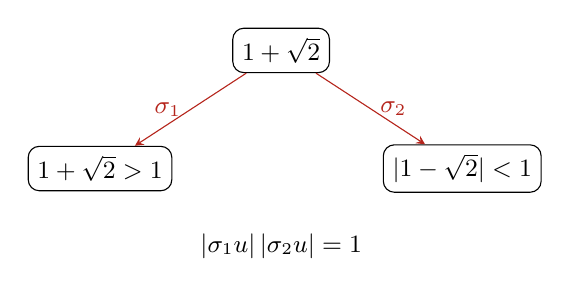
\begin{tikzpicture}[>=stealth,font=\small]
\node[draw,rounded corners] (u) at (0,0) {$1+\sqrt2$};
\node[draw,rounded corners] (a) at (-2.3,-1.5) {$1+\sqrt2>1$};
\node[draw,rounded corners] (b) at (2.3,-1.5) {$|1-\sqrt2|<1$};
\draw[->,BrickRed] (u)--node[left] {$\sigma_1$}(a);
\draw[->,BrickRed] (u)--node[right] {$\sigma_2$}(b);
\node[below] at (0,-2.2) {$|\sigma_1u|\,|\sigma_2u|=1$};
\end{tikzpicture}
